\documentclass[10pt, conference, letterpaper]{IEEEtran}

\usepackage{graphicx}
\usepackage{amsmath}
\usepackage{amssymb}
\usepackage{booktabs}
\usepackage{subcaption}
\usepackage{url}

\graphicspath{{./figures/}}

\begin{document}

\title{Sunflower Robot: A Solar-Tracking Robot with Custom Mechanics and Closed-Loop Light Seeking}
\IEEEoverridecommandlockouts
\author{Alexandru Mihailescu\thanks{Work done for the course of Modelling and Control of Electric Drives, taught by Prof. Nicola Bianchi at the University of Padua.}}

\maketitle

\begin{abstract}
The objective was a two-axis solar tracker built almost entirely from parts already in storage and from 3D-printed mechanics, able to point an array of small solar panels at the brightest light source in the room. The approach combined a characterisation of the light sensor, a custom high-ratio spur gearbox designed in OpenSCAD with the BOSL2 library, a printed body designed in Autodesk Fusion, and a closed-loop tracking algorithm that follows the gradient of the measured luminosity rather than a fixed reference. The final build tracks light on both axes: it detects the direction of increasing intensity, drives towards it, and stops and backs up as soon as the intensity drops. Two failures dominated the effort: a first gearbox whose friction stalled the original 6\,V motors, which forced a redesign around 12\,V motors and fewer, larger gears; and a soldering-induced fault in the analogue front end, compounded by a capacitor-like charge and discharge behaviour in one solar panel, which forced the differential two-panel sensing scheme to be abandoned in favour of a single aggregated luminosity channel.
\end{abstract}

\section{Introduction and Objective}

The goal of the project was to design and build a robot carrying solar panels and DC motors, capable of tracking a light source in order to maximise the energy it produces. Two self-imposed constraints shaped every decision that follows:

\begin{itemize}
  \item only electrical and mechanical components already available from previous hobby kits and from storage were to be used;
  \item the body and most of the moving parts were to be 3D-printed.
\end{itemize}

The ambition was a cheap, feasible and custom-made solution. Most of the 3D modelling was done in Autodesk Fusion. Gear generation was done in OpenSCAD with the BOSL2 library.

The report is organised by engineering phase. Section~\ref{sec:sensor} characterises the light sensor and fixes the form of the control law. Section~\ref{sec:mech} covers the mechanical design and the gearbox. Section~\ref{sec:proto} covers gearbox prototyping and the iterations forced by test failures. Section~\ref{sec:elec} covers the electronics and the integration problems. Section~\ref{sec:algo} describes the tracking algorithm and the filtering. Sections~\ref{sec:results} and~\ref{sec:concl} give the results and the conclusions.

\section{Sensor Characterisation}
\label{sec:sensor}

\subsection{Photoresistor response to angle}

Before committing to a sensor, the first question was what the output of a single light sensor looks like as a light source sweeps across it. The answer determines what kind of algorithm can find the brightest direction.

The setup was deliberately simple. A photoresistor was held in a fixed position. A torch was moved above a protractor printed on an A4 sheet and rotated through known angles. The photoresistor, whose measured resistance ranged from a maximum of $38\,\mathrm{k}\Omega$ to a minimum of $132\,\Omega$, was placed in a voltage divider across 5\,V with the ADC of an Arduino Uno connected to the midpoint. At each angle the Arduino averaged a few samples, converted the ADC counts to volts, and sent the result over the serial monitor, where it was recorded by hand.

The result is shown in Fig.~\ref{fig:sensor-response}. The divider voltage is low where the light is strongest, which confirms that the resistance of the photoresistor is inversely proportional to the light it receives. More useful than the sign is the shape: the signal rises rapidly away from the peak and then stalls towards its extreme. The measurement is indicative only, since the photoresistor is non-linear, exhibits a hysteresis cycle, and carries considerable measurement uncertainty at low luminosity.

\begin{figure}[!t]
  \centering
  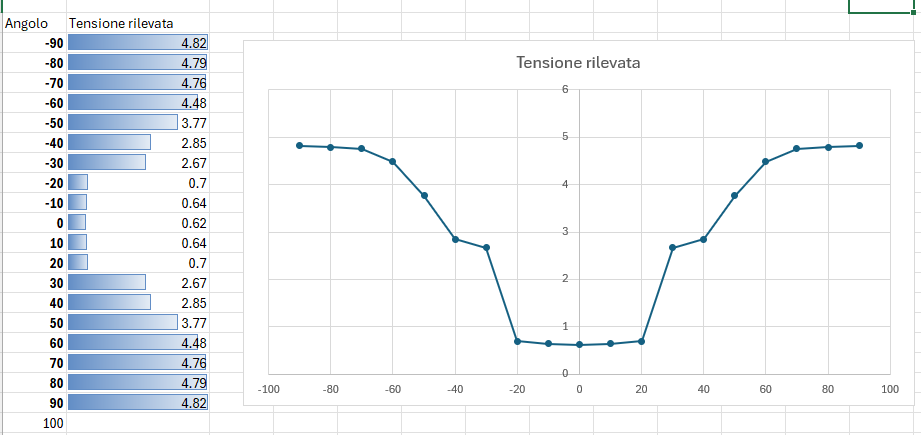
\includegraphics[width=\columnwidth]{sensor-response-angle}
  \caption{Divider voltage against torch angle over the protractor. The response saturates away from the peak and is far from linear.}
  \label{fig:sensor-response}
\end{figure}

\subsection{Consequence for the control law}

A signal of this shape has no fixed reference value to regulate against, but it does have a well-defined maximum. That suggests a scheme analogous to gradient descent: drive the axis while the luminosity keeps improving, and as soon as the movement takes the sensor away from the maximum, stop and back up to the previous best point. The same rule applies unchanged to the up and down axis and to the clockwise and counterclockwise axis. This idea survived into the final implementation.

Post-processing of the same data (Fig.~\ref{fig:sensor-transforms}) showed that a logarithmic transform sharpens small differences in the readings and could improve discrimination near the peak. The quality of the manually acquired data was not sufficient to confirm that the gain would be practical, so the question was deferred until a working prototype could produce better data.

\begin{figure}[!t]
  \centering
  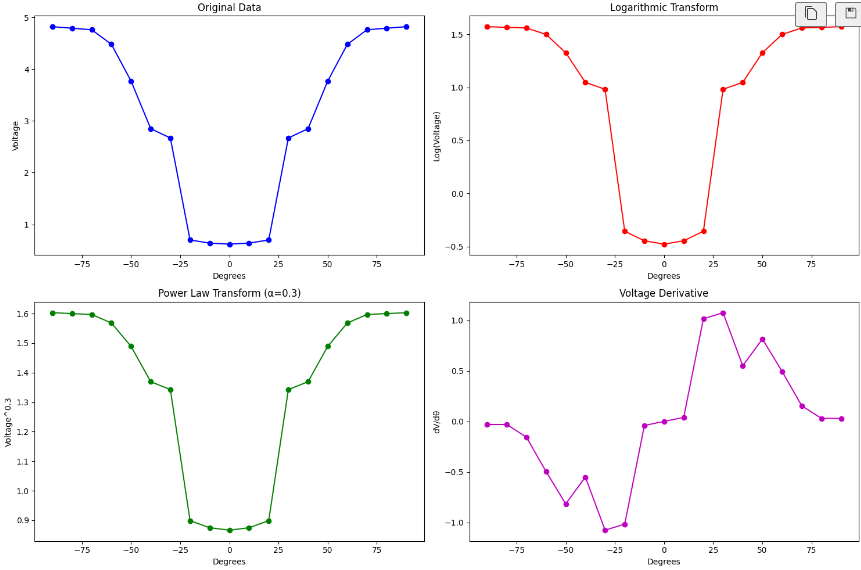
\includegraphics[width=\columnwidth]{sensor-transform-tests}
  \caption{Transform tests on the acquired data: raw signal, logarithmic transform, power law transform, and the derivative with respect to angle.}
  \label{fig:sensor-transforms}
\end{figure}

\subsection{From photoresistor to solar panels}

The panels bought for the project are rated 3\,V and 0.3\,W, measuring $65 \times 48$\,mm, in a pack of six. Since the voltage of a panel is proportional to the light it receives, the panels themselves can serve as the sensor and remove the need for a separate photoresistor in the final build. Measured against the artificial light sources available, the panels reached up to 3.6\,V at maximum luminosity.

Six panels admit either a flat rectangular layout or something more articulated. The angular characterisation above showed that even a flat rectangular layout would give a usable reading, so a petal layout was chosen instead, for two reasons: it matches the sunflower concept, and it places panels in opposite positions so that the difference between two of them can supply directional information. Two panels were connected to analogue inputs of the Arduino and to ground, each with a $100\,\mathrm{k}\Omega$ resistor in parallel. The remaining panels were left disconnected, pending a charging module that would put the generated power to use.

\section{Mechanical Design and Gearbox}
\label{sec:mech}

\subsection{Actuation requirement}

The DC motors already available were rated 1.5\,V to 6\,V with a no-load speed of 20\,000\,RPM. Moving the panel array slowly and steadily against the friction and inertia of the assembly is impossible at that speed and torque, so a transmission was mandatory. It was later realised as a spur gearbox with a very high reduction ratio. Fig.~\ref{fig:controller-sketch} shows the first sketch of the electrical configuration around the controller, at a point where a discrete transistor H-bridge was still the intended motor drive.

\begin{figure}[!t]
  \centering
  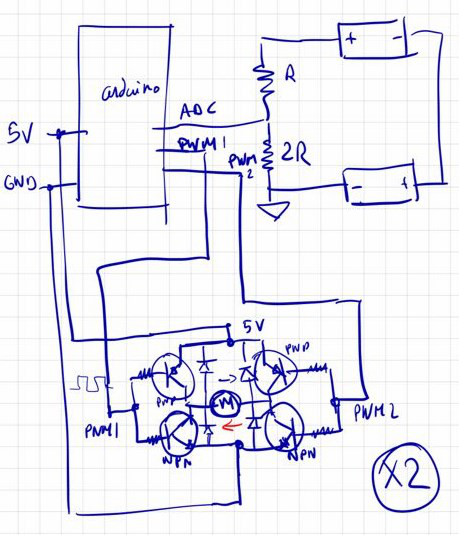
\includegraphics[width=0.85\columnwidth]{controller-sketch}
  \caption{First sketch of the basic electrical configuration of the controller, with the discrete transistor H-bridge originally intended for the motor drive.}
  \label{fig:controller-sketch}
\end{figure}

\subsection{Constraints imposed by the printing process}

Every mechanical decision in the project is bounded by what fused deposition modelling can produce. The printer used was a modified Creality Ender 3, with a build volume of $220 \times 220 \times 250$\,mm and a nozzle able to hold a stable 240\,$^{\circ}$C. Models were exported to STL, sliced in PrusaSlicer into layer-by-layer toolpaths (Fig.~\ref{fig:slicer}), and printed in PETG, chosen for its mechanical strength and low cost. Both properties mattered, because many prototypes of many small components were going to be needed.

\begin{figure}[!t]
  \centering
  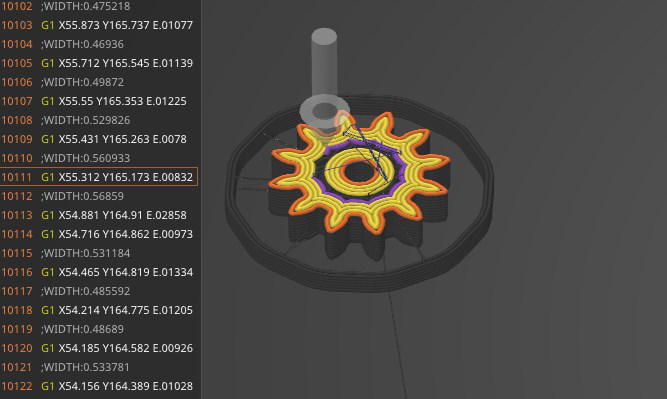
\includegraphics[width=\columnwidth]{slicer-preview}
  \caption{Slicer preview of the toolpath commands for a printed gear.}
  \label{fig:slicer}
\end{figure}

The parts must adhere to a heated bed and must be constructible layer by layer, which restricts the shapes that can be designed at all. The concrete consequences on this design were:

\begin{itemize}
  \item the 0.2\,mm nozzle sets the achievable tolerance, and therefore the minimum practical tooth size and count;
  \item gear width could not be reduced freely, because the first layer is squashed against the bed and the resulting deformation dominates the friction budget of a thin gear;
  \item layer height is a trade-off, since thinner layers mean more squashing and warping but also better interlayer bonding and stronger parts, and the balance had to be found empirically;
  \item the outer walls of the gearboxes were held to at least 2.5\,mm to survive the forces in play.
\end{itemize}

\subsection{Concept and axes}

The layout follows the sunflower directly (Fig.~\ref{fig:concept}). The petals are the solar panels, and the sensing scheme described above uses two opposite petals.

\begin{figure}[!t]
  \centering
  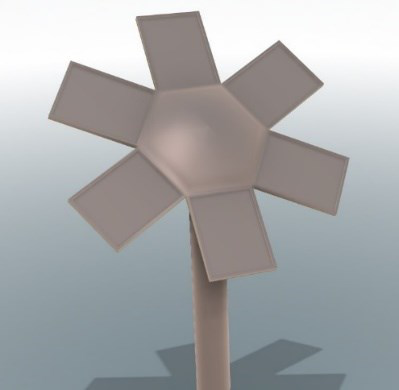
\includegraphics[width=0.7\columnwidth]{concept-flower}
  \caption{First concept of the Sunflower, with the panels arranged as petals.}
  \label{fig:concept}
\end{figure}

Vertical rotation (up and down of the flower head) is produced by a column of gears sitting on the main axis, which is therefore split in two halves joined by metal rods that also support the gears. The column transmits motion from the base, where both DC motors and the Arduino sit.

Horizontal rotation had to avoid interfering with the mechanics and electronics already on the base. The solution was to place the whole flower on a bearing locked to a lower base, allowing free 360$^{\circ}$ rotation, and to drive that rotation from the second DC motor through its own reduction stage, to raise torque and lower speed enough for fine positioning. Fig.~\ref{fig:rotation-sketch} shows the early sketch of the two axes.

\begin{figure}[!t]
  \centering
  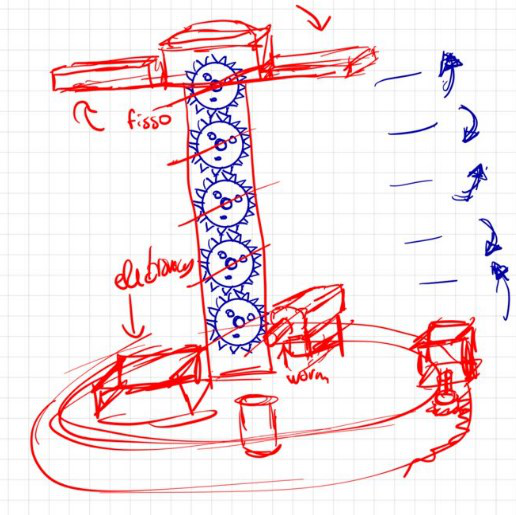
\includegraphics[width=0.8\columnwidth]{rotation-sketch}
  \caption{Early sketch of the vertical gear column and of the horizontal base rotation.}
  \label{fig:rotation-sketch}
\end{figure}

\subsection{Gear design}

A large share of the mechanical effort went into gear design equations, and into printing and testing gear prototypes (Fig.~\ref{fig:printed-gears}). Autodesk Fusion has a gear toolkit, but it could not accommodate the hard constraints of this build: the bores had to match the diameters and tolerances of parts already owned, while the pitch diameters and tooth counts had to hit specific values dictated by the reduction ratio and by the available space. Working within those constraints made it necessary to understand the underlying standards and equations rather than rely on the toolkit. Together with the tolerance floor set by the nozzle, this forced repeated redesign and rescaling of the gears so that they would mesh cleanly and sit on their axes without binding or slop. The solution adopted for the rest of the project was the BOSL2 library for OpenSCAD, which gave far more control than Fusion, and generated every gear used in the final build.

\begin{figure}[!t]
  \centering
  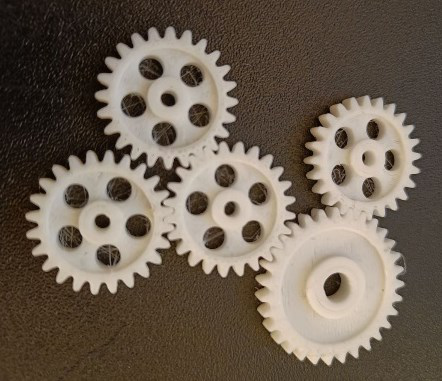
\includegraphics[width=0.75\columnwidth]{printed-gears}
  \caption{A sample of the many gears printed and tested during the project.}
  \label{fig:printed-gears}
\end{figure}

An attempt was also made to move the CAD work from Fusion to FreeCAD, an open-source alternative, in order to escape the limitations of Fusion. The workflows differ enough that the learning curve cost more than working around those limitations, so the attempt was abandoned. This was the first CAD project of this scale attempted, with no previous familiarity with 3D design workflows, which made the switch more expensive than it would otherwise have been.

\subsection{Shafts and recovered hardware}

The vertical gears run on M3 screws already in storage. The remaining shafts, namely those holding the gears inside the gearboxes, the main wooden top axis, and the shaft between the bearing and the lower base, are spare parts left over from IKEA products (Fig.~\ref{fig:ikea}). IKEA supplies small parts for free or very cheaply against a part code, and keeps them available across decades and across many products, which makes them both a good use of leftovers and a sustainable choice, since a broken shaft is trivially and cheaply replaced.

\begin{figure}[!t]
  \centering
  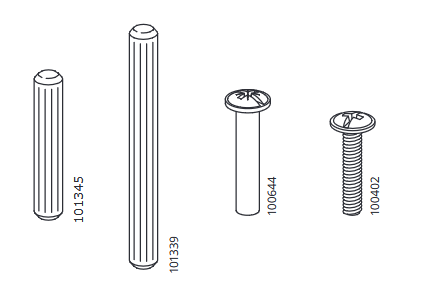
\includegraphics[width=0.8\columnwidth]{ikea-parts}
  \caption{The recovered IKEA parts used as shafts.}
  \label{fig:ikea}
\end{figure}

\begin{table}[!t]
  \caption{Recovered shafts and their function}
  \label{tab:parts}
  \centering
  \begin{tabular}{@{}lll@{}}
    \toprule
    Part & Source & Function \\
    \midrule
    101345 & BEST system & Bearing shaft to the lower base \\
    101339 & KALLAX shelving & Main axis of the final vertical gear \\
    100644 + 100402 & Pax/Forsand & Main axis of the gearboxes \\
    \bottomrule
  \end{tabular}
\end{table}

The choices in Table~\ref{tab:parts} were driven by load. A PETG shaft as small as the available bearing would not have survived the weight of the robot standing above it, so part 101345 was used instead. The wooden part 101339 carries the torque from the last vertical gear to the pistil, the platform on which the panels are mounted. Parts 100644 and 100402 screw into each other and are stainless steel, which made them ideal as the gearbox main axis despite the extra difficulty introduced by their larger diameter. Given the ratios involved in the initial designs, that was a necessary choice for structural integrity during operation.

From this point on, every design decision had to accommodate these parts as well as the printer. The length of the gearbox axis caps the space available for gears, which caps their number and width, and forces a compromise: fewer, larger gears, or more, slimmer gears with a higher total ratio.

\section{Gearbox Prototyping and Iteration}
\label{sec:proto}

\subsection{First prototype and its failure}

With those constraints in place, an optimistic first gearbox was designed with a reduction ratio of about 638 and printed (Figs.~\ref{fig:gearbox-v1} and~\ref{fig:gearbox-v1-int}). It was tested in the lab on a bench DC supply, since no supply at home delivered enough power.

\begin{figure}[!t]
  \centering
  \begin{subfigure}[b]{0.46\columnwidth}
    \centering
    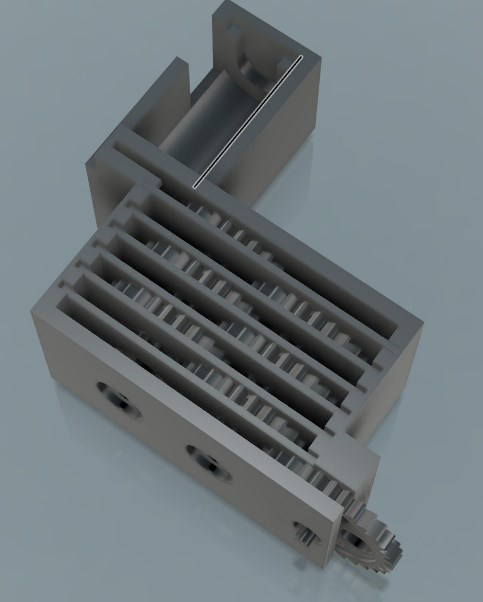
\includegraphics[width=\linewidth]{gearbox-v1}
    \caption{}
    \label{fig:gearbox-v1}
  \end{subfigure}
  \hfill
  \begin{subfigure}[b]{0.5\columnwidth}
    \centering
    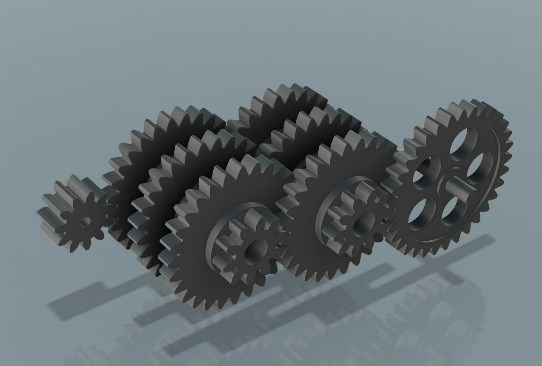
\includegraphics[width=\linewidth]{gearbox-v1-interior}
    \caption{}
    \label{fig:gearbox-v1-int}
  \end{subfigure}
  \caption{First gearbox prototype, with the housing shaped around the DC motor already owned (a), and the interior view of the gear train (b).}
\end{figure}

The test failed, and the failure was informative. The 6\,V motor did not start even when supplied with the maximum available current and driven at 12\,V. It overheated and began to fume. The gearbox itself could be turned by finger, but its friction was too high and its tolerances too tight for the motor to break it loose. A silicon-based lubricant between the gears, the inner walls and the axes was not enough.

Three conclusions followed, and each drove a change:

\begin{enumerate}
  \item the motors were underpowered and had to be replaced;
  \item the number of moving parts had to come down;
  \item friction had to be attacked directly in the geometry.
\end{enumerate}

For the third point, small rings of material were added to reduce the contact area between the gears and the inner walls (Fig.~\ref{fig:wall-redesign}). Slightly increasing the root diameter of the gears allowed the gear count to be reduced while keeping a comparable output ratio.

\begin{figure}[!t]
  \centering
  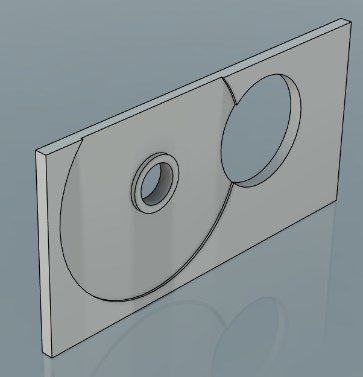
\includegraphics[width=0.6\columnwidth]{gearbox-wall-redesign}
  \caption{Redesign of the gearbox inner wall, with rings that reduce the contact area between gears and walls.}
  \label{fig:wall-redesign}
\end{figure}

Two 12\,V motors were procured to replace the 6\,V hobby-kit motors. At the same time the discrete transistor H-bridge originally planned was dropped in favour of an L298N dual H-bridge module (Fig.~\ref{fig:motors}), to cut complexity and shorten the path to a working system.

\begin{figure}[!t]
  \centering
  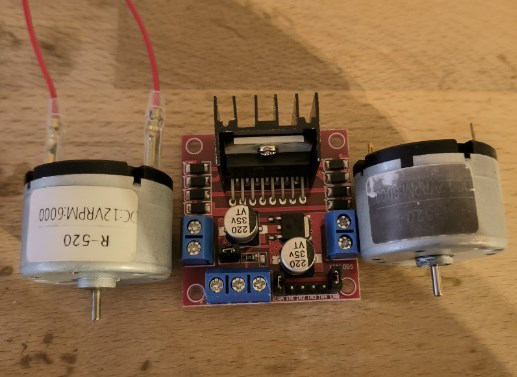
\includegraphics[width=0.8\columnwidth]{motors-l298n}
  \caption{The 12\,V motors and the L298N dual H-bridge module that replaced the 6\,V motors and the planned discrete bridge.}
  \label{fig:motors}
\end{figure}

\subsection{Second and third gearbox}

A full redesign of the gearbox and its gears was expensive, so an incremental second iteration was tried first: the same architecture with the friction fixes described above. Printed complete with gears and inner walls, it still failed to run. That result proved the new motors were necessary.

The gearbox was then completely redesigned around a smaller number of gears and the two new motors, and a third prototype was printed. This one worked. Rotation was smooth, if loud. Gears and gearbox internals were left deliberately exposed as a design choice, as were the vertical axis gears.

\subsection{Vertical axis and pistil}

The vertical axis was then designed with seven gears, chosen so that the pistil turns in the same direction as the output gear of the gearbox (Figs.~\ref{fig:vaxis} and~\ref{fig:vaxis-test}). The pistil, the part that carries the panels, could not be printed as a single piece within the build volume, so the panel frames were made separate parts screwed into it. That split turned out to be useful later, when the pistil was redesigned, because reprinting it did not mean reprinting the frames. Each panel is held by three 3\,mm screws, with the holes in the pistil and in the frames oriented at about 30$^{\circ}$ to improve structural rigidity.

\begin{figure}[!t]
  \centering
  \begin{subfigure}[b]{0.44\columnwidth}
    \centering
    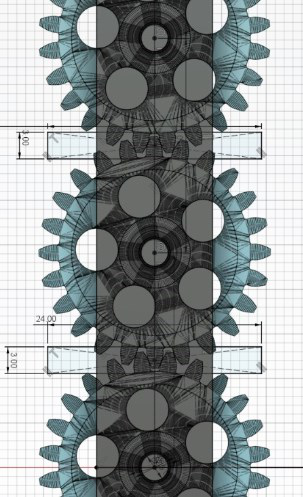
\includegraphics[width=\linewidth]{vertical-axis-section}
    \caption{}
    \label{fig:vaxis}
  \end{subfigure}
  \hfill
  \begin{subfigure}[b]{0.44\columnwidth}
    \centering
    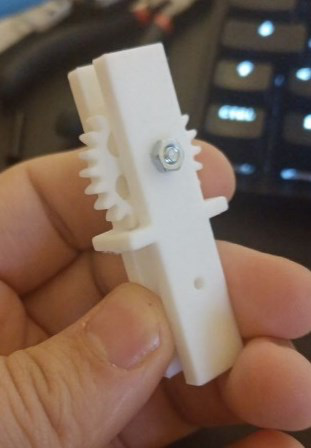
\includegraphics[width=\linewidth]{vertical-axis-test-print}
    \caption{}
    \label{fig:vaxis-test}
  \end{subfigure}
  \caption{See-through view of the first version of the vertical axis (a), and a small section of it printed on its own to check tolerances (b).}
\end{figure}

\subsection{Base rotation}

The base rotation was the hardest part to design, because the strength of the printed material ruled out most of the obvious solutions. The feasible one connects the output of the gearbox directly to the lower base, transmitting rotation through a cut in the upper base and in the gearbox. That gear drives a custom double gear held inside a ring screwed to the upper base; by rolling on the lower base it turns the upper base. The upper base rests with all its weight on the bearing, and is located both by the printed material and by the wooden axis (Figs.~\ref{fig:upper-base} and~\ref{fig:lower-base}).

\begin{figure}[!t]
  \centering
  \begin{subfigure}[b]{\columnwidth}
    \centering
    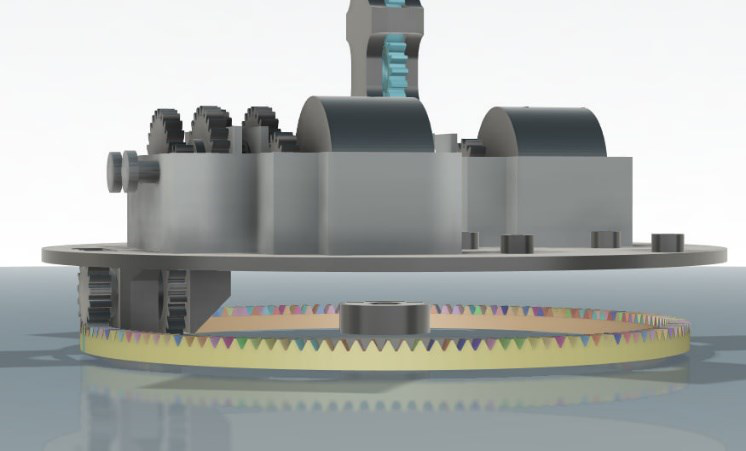
\includegraphics[width=0.95\linewidth]{upper-base}
    \caption{}
    \label{fig:upper-base}
  \end{subfigure}

  \vspace{2mm}
  \begin{subfigure}[b]{\columnwidth}
    \centering
    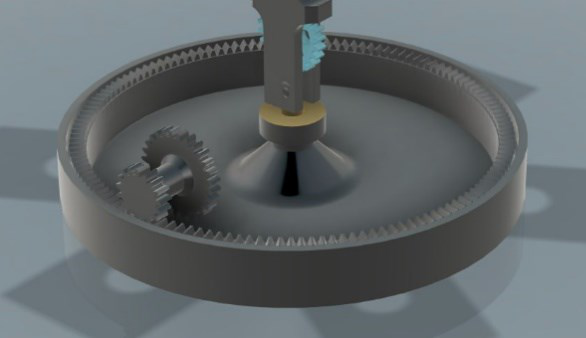
\includegraphics[width=0.95\linewidth]{lower-base}
    \caption{}
    \label{fig:lower-base}
  \end{subfigure}
  \caption{Upper base with gearboxes and vertical axis mounted, horizontal rotation gear visible against the lower base ring (a), and the lower base with the upper base gear and the vertical axis in view (b).}
\end{figure}

\begin{figure}[!t]
  \centering
  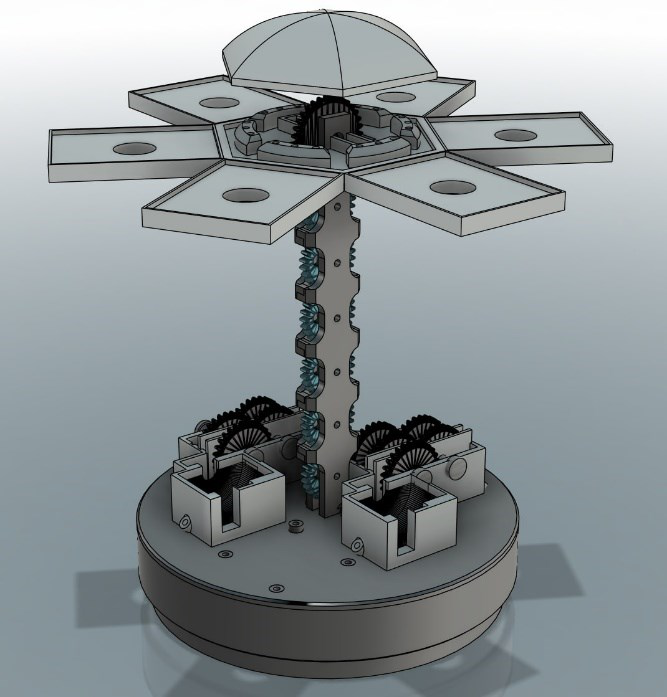
\includegraphics[width=0.9\columnwidth]{prototype-design-v1}
  \caption{First complete prototype design of the Sunflower robot.}
  \label{fig:proto-v1}
\end{figure}

\subsection{Iterations forced by the physical build}

Sections of the design were printed and assembled incrementally to verify tolerances before committing to the full robot. Three problems only became visible once real parts were in hand, and each forced a rework.

\textbf{The pistil blocked its own rotation.} Only after the pistil was fully built did it become clear that the shape and size of the panels and of the frame holding them severely obstructed the up and down rotation. The pistil was therefore split into two parts held together by the wooden axis, which is locked into both (Fig.~\ref{fig:pistil-v2}). The second version allows a full 90$^{\circ}$ rotation in each direction, so 180$^{\circ}$ of travel for the panels. The only remaining obstruction is the stiffness of the panel cables, which had to be resoldered with thinner wire to cut friction and weight.

\begin{figure}[!t]
  \centering
  \begin{subfigure}[b]{0.48\columnwidth}
    \centering
    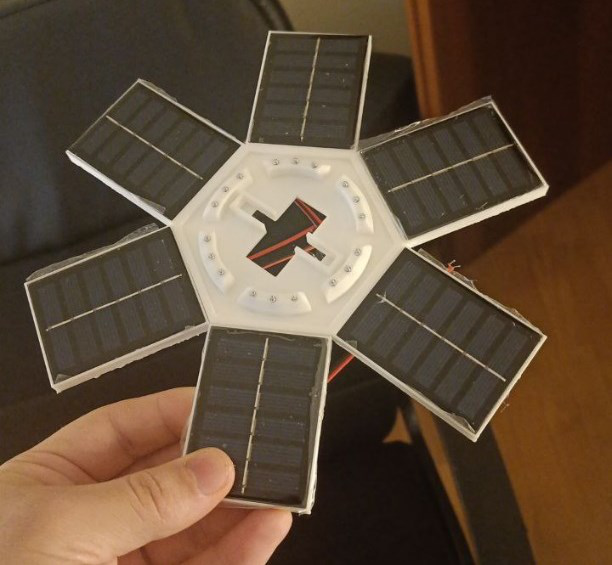
\includegraphics[width=\linewidth]{pistil-v1-print}
    \caption{}
    \label{fig:pistil-v1}
  \end{subfigure}
  \hfill
  \begin{subfigure}[b]{0.48\columnwidth}
    \centering
    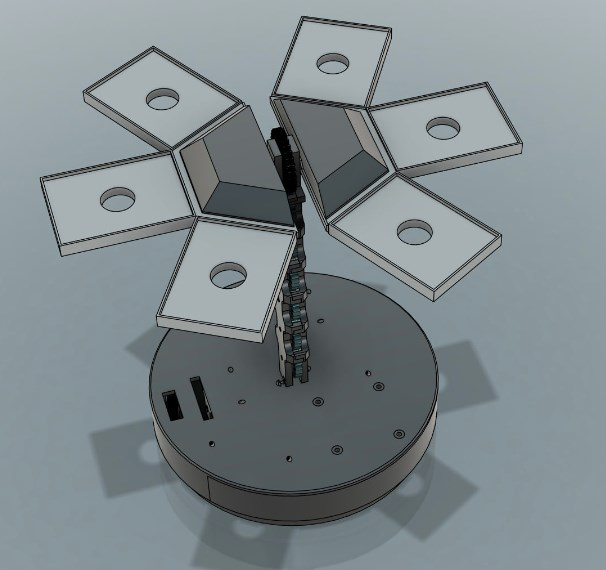
\includegraphics[width=\linewidth]{pistil-v2}
    \caption{}
    \label{fig:pistil-v2}
  \end{subfigure}
  \caption{First version of the pistil frame with the panels and their frames mounted (a), and the second iteration with the split pistil that clears the full 180$^{\circ}$ of travel (b).}
\end{figure}

\textbf{The bearing could not carry the load.} With the second pistil, the base, the axis, the second gearbox and the lower base assembled, the bearing was clearly unable to bear the weight of the upper structure. It allowed the upper assembly to rock, which made horizontal rotation unstable and imprecise. Rather than overhaul the upper base, three additional mixed gears were fixed to the upper base and positioned between the upper and lower base (Fig.~\ref{fig:upper-base-v2}). They support the load and block the wobble. The part is large and expensive to print, but still cheaper than a full redesign of the upper base.

\begin{figure}[!t]
  \centering
  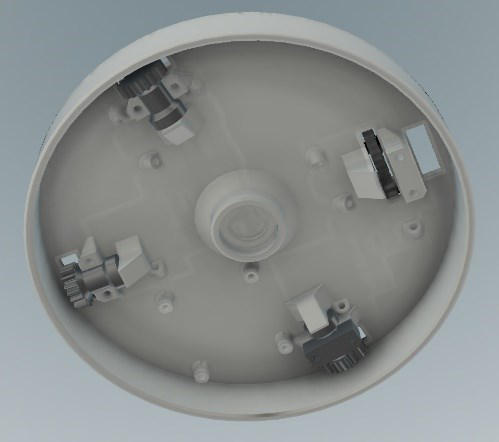
\includegraphics[width=0.7\columnwidth]{upper-base-v2-underside}
  \caption{Second iteration of the upper base seen from below, with the three added mixed gears that carry the load and block the wobble.}
  \label{fig:upper-base-v2}
\end{figure}

\textbf{Backlash in the vertical axis.} Small tolerance errors between the designed and the printed gears accumulate along the vertical gear column, producing a visible delay between the rotation of the motor shaft and the rotation of the pistil. The fix was to scale the vertical axis gears up slightly, by 1\,\% or less, which reduces the gap between meshing teeth. It took a few prints per gear to converge, and it improved the response of the pistil enough to be acceptable. Fig.~\ref{fig:final-render} shows the resulting mechanical design.

\begin{figure}[!t]
  \centering
  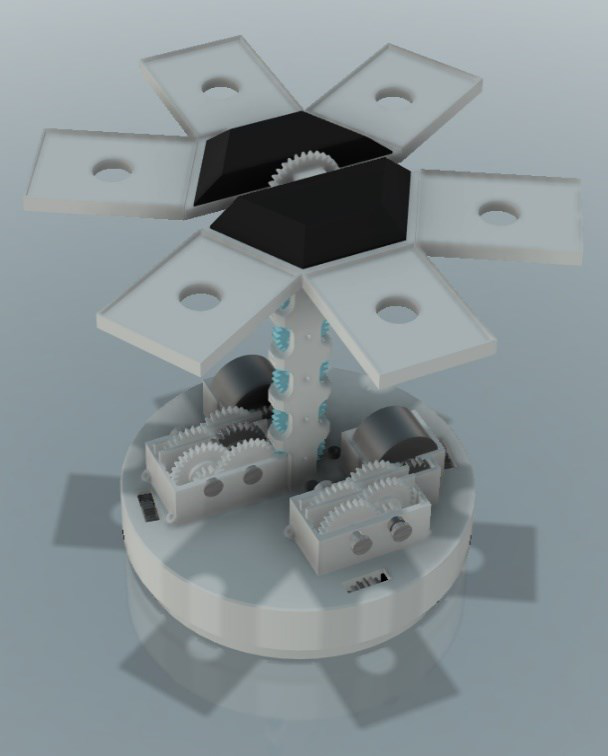
\includegraphics[width=0.85\columnwidth]{final-design-render}
  \caption{Final design of the Sunflower robot, shown without the electrical components and the solar panels.}
  \label{fig:final-render}
\end{figure}

\section{Electronics and Integration}
\label{sec:elec}

\subsection{Analogue front end and filtering}

Artificial light sources in the room flicker at roughly 50\,Hz, and that flicker was visible in the first readings. Each panel output was therefore passed through a passive low-pass filter with a cutoff of about 16\,Hz. The cutoff was not set lower on purpose: a lower cutoff would introduce more than 10\,ms of delay, which would degrade the response of the motors during a movement.

\subsection{Power supply fault}

The first algorithm tests were corrupted by a failing bench supply. It kept delivering power, but in an anomalous and unpredictable way, at varying frequency. The fault was only identified because the two panel signals stopped being consistent with each other, which is also what motivated a proper calibration experiment. A replacement supply was built from an old laptop adapter, with its ends adapted to a breadboard and to the motor driver, and with a custom printed plastic enclosure for a power button.

\subsection{Permanent build and the soldering fault}

With the software working and the parts working together, the circuit was moved off the breadboard into a permanent build: the panels were glued to their frames, and an Arduino Nano V3 was soldered, together with the passive filters and the new panel wiring, onto a blank circuit board. The Nano is far less bulky than the Uno used on the prototype. Every connection was checked with a multimeter to confirm that each panel presented the right voltage to the right port, cable routing was chosen so as not to obstruct the movement of the robot, and every new joint was insulated with heat shrink sleeving and hot glue to keep added electrical noise low.

After reassembly, nothing worked as before. On the Arduino IDE plotter the signals looked as if they had been scaled or offset by some factor (Figs.~\ref{fig:hysteresis} and~\ref{fig:recal}). The first hypothesis was that resoldering the panel cables had changed some resistance in the divider. Repeated cycles of acquiring calibration data, fitting a compensation function and testing did not converge: the behaviour of the panels appeared to change slightly on every run, no matter how much data was used or how tightly the acquisition conditions were controlled. Without an oscilloscope, diagnosis was largely guesswork, since the ADC ports and the serial plotter give very little insight into an analogue fault.

\begin{figure}[!t]
  \centering
  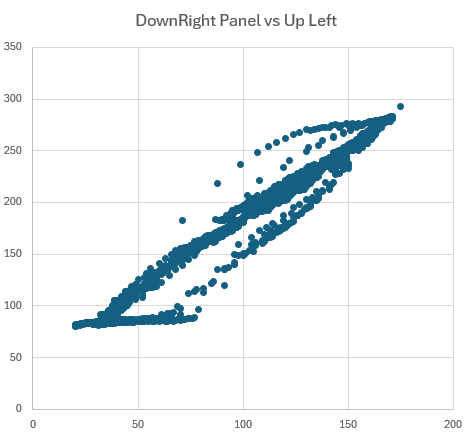
\includegraphics[width=0.75\columnwidth]{panel-hysteresis}
  \caption{Calibration data acquired after the permanent build. One panel plotted against the other traces a loop rather than a curve, which is the signature of the charge and discharge behaviour later identified.}
  \label{fig:hysteresis}
\end{figure}

\begin{figure}[!t]
  \centering
  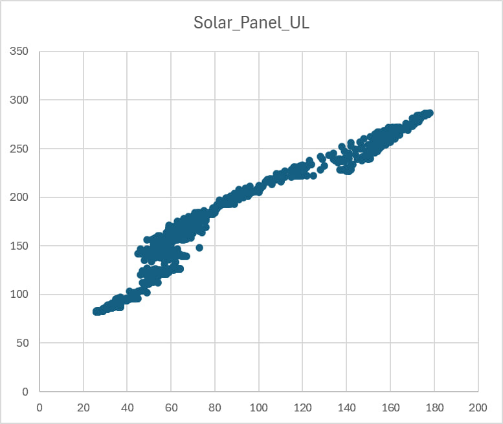
\includegraphics[width=0.75\columnwidth]{panel-recalibration}
  \caption{A further calibration set acquired under nominally identical conditions. The relationship shifts between runs.}
  \label{fig:recal}
\end{figure}

Two causes were eventually found, and they are additive.

\textbf{A damaged filter capacitor.} The suspicion arose that one of the capacitors in the passive filters had been destroyed by heat during soldering. With the remaining solder, the physical filters were removed and the panels were connected directly to the ADC, with software filters substituting for the missing hardware. The data driving the robot was still noisy, but the behaviour of the robot returned close to what it had been before the soldering.

\textbf{Charge and discharge behaviour in a panel.} The remaining erratic behaviour was explained in the lab, under much brighter light than was ever available at home: direct sunlight plus multiple fluorescent fixtures. Under that illumination one of the panels visibly charged and discharged like a capacitor, adding a term to its voltage that does not correspond to the instantaneous light. The tracking algorithm did not account for it, and under those conditions the tracking became more erratic than before.

\subsection{Final front end}

Disassembling the robot to rewire the panels would have cost more than the remaining budget allowed. The cheaper path exploited hardware that was already in place: the four unused panels were already connected in series and routed to the Arduino board, in view of a future power measurement circuit. They were connected to a newly soldered low-pass filter (soldered quickly and carefully to avoid destroying another capacitor) and to a voltage divider, and fed to an ADC port that had never been used, so that no fault in the old ports could carry over. This gives a single aggregated luminosity channel instead of two differential ones. It sacrifices directional awareness, but it is sound, and it is what the final firmware uses.

\begin{table}[!t]
  \caption{Final electrical configuration}
  \label{tab:elec}
  \centering
  \begin{tabular}{@{}ll@{}}
    \toprule
    Item & Value \\
    \midrule
    Controller & Arduino Nano V3 \\
    Motor drive & L298N dual H-bridge \\
    Motors & 2 $\times$ 12\,V DC \\
    Panels & 6 $\times$ 3\,V, 0.3\,W, $65 \times 48$\,mm \\
    Sensing & 4 panels in series, low-pass filter, divider, one ADC \\
    Supply & Modified laptop adapter \\
    \bottomrule
  \end{tabular}
\end{table}

\section{Control Algorithm}
\label{sec:algo}

\subsection{Why not a PID}

A PID controller was considered first and discarded. Light tracking of this kind offers no fixed reference value to regulate against: the objective is to maximise an unknown, drifting quantity, not to hold it at a setpoint. The extremum-seeking scheme identified during the sensor characterisation does not need a reference, which is why it was adopted.

\subsection{Differential scheme and panel calibration}

The first implementation added directional awareness to the basic scheme: instead of only checking whether the luminosity is descending, the robot maximised the light received by the two connected panels while minimising the difference between their readings. That only works if the two panels are matched, and they are not.

To calibrate them, a LED strip was glued to a wooden plank and driven from a dimmer, and data was acquired continuously from both panels with a Python script and written to CSV (Fig.~\ref{fig:calib-setup}). The panel outputs were filtered as described in Section~\ref{sec:elec} before acquisition. The experiment demands complete darkness and stable light, and it took several attempts to suppress interference from light reflected off walls and furniture. The data was then cleaned, selected and processed in Microsoft Excel, leaving 773 samples per panel, acquired at light levels raised and then lowered again in steps. A photoresistor served as the reference, with the luminosity in lux computed from the manufacturer's datasheet.

\begin{figure}[!t]
  \centering
  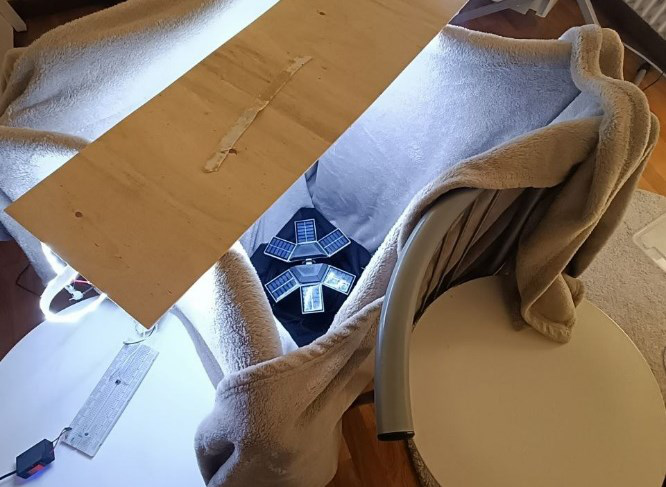
\includegraphics[width=0.85\columnwidth]{calibration-setup}
  \caption{Setup used to acquire the calibration data: LED strip on a plank, dimmer, and the robot shielded from ambient light.}
  \label{fig:calib-setup}
\end{figure}

Modelling panel voltage directly against lux (Fig.~\ref{fig:panel-lux}) proved impractical. Uncertainty at low light levels made the data hard to fit, and the polynomial degree required was high enough to compromise the acquisition rate given the compute available on the Arduino.

\begin{figure}[!t]
  \centering
  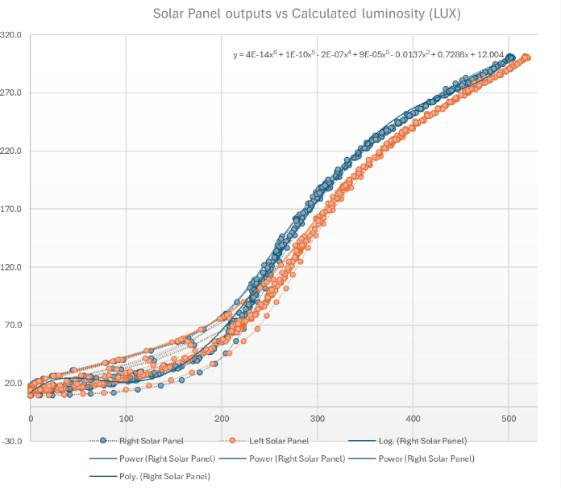
\includegraphics[width=0.9\columnwidth]{panel-output-vs-lux}
  \caption{Outputs of the two solar panels against the luminosity computed from the reference photoresistor.}
  \label{fig:panel-lux}
\end{figure}

The practical alternative was to model the difference between the panels at equal illumination. Once that difference is modelled, one panel can be compensated so that its readings resemble what the other would report for the same luminosity, which makes the difference between the two readings usable as a direction cue for both axes.

Even the difference resisted a single polynomial fit. Since its behaviour changes above a certain luminosity, the data was split in two at that value and fitted with two separate polynomial regressions, with a threshold in the Arduino code selecting the model to apply (Fig.~\ref{fig:compensation}). Splitting the models and applying the compensation immediately improved the signals observed from the Arduino. The minimisation of the difference was then straightforward to implement for the vertical axis and then for the horizontal one.

\begin{figure}[!t]
  \centering
  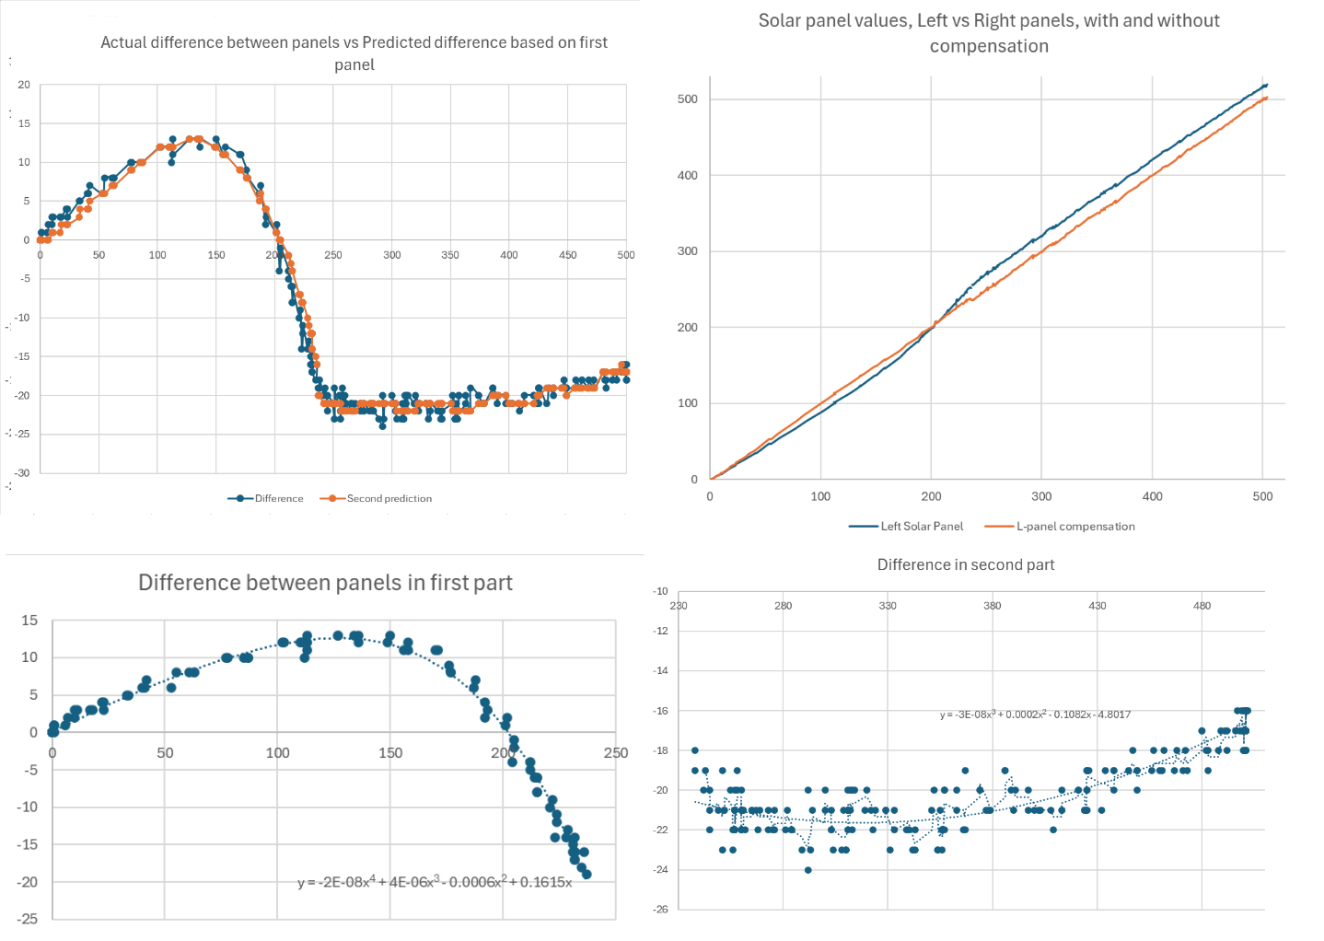
\includegraphics[width=\columnwidth]{panel-compensation}
  \caption{Panel compensation. Top left: measured difference between the panels against the difference predicted from the first panel. Top right: left panel before and after compensation. Bottom: the two piecewise polynomial fits of the difference, below and above the split threshold.}
  \label{fig:compensation}
\end{figure}

This scheme was validated on the vertical axis on the prototype. It was abandoned only because of the analogue faults described in Section~\ref{sec:elec}, not because of a defect in the scheme itself.

\subsection{Final scheme: gradient ascent on a single channel}

The firmware that ships with this report (\texttt{firmware/Sunflower\_project\_V5.ino}) drives both axes from the single aggregated luminosity channel. It is a direct implementation of the extremum-seeking idea formed during the sensor characterisation.

\emph{Measurement.} Each ADC sample is fed into an 8-sample moving average. All waiting in the firmware is done inside loops that keep sampling and keep the average current, so the controller never acts on a stale reading. The moving average holds the residual noise at roughly $\pm 1$ count.

\emph{Trigger.} The main loop compares the current average against the best luminosity seen so far. If it has fallen below 93\,\% of that maximum, the light has moved and a tracking action is started. Between checks the loop idles. The idle interval is short in the firmware for testing, and would be set to something on the order of an hour in a real deployment.

\emph{Search.} An axis is driven in one direction while the luminosity is monitored continuously. The direction is judged wrong, and the motor stopped, as soon as the average falls more than 3 counts below the best value seen during that movement, a dead band that keeps sensor noise from ending the sweep prematurely. While the reading improves, the running best and the global maximum are updated. Under lab conditions, where the light can also move backwards, the opposite direction is then swept in the same way, and the axis finally backs up towards the position where the maximum was seen. The global maximum is reset to the value reached at the end of the action, so that any later change in the light is detected against the new operating point.

\emph{Actuation.} The motors are driven by PWM through the L298N. Duty cycle is bounded below by the friction of the drive train and above by the need to keep the search resolvable: 35\,\% minimum for the horizontal axis, 28\,\% minimum for the vertical axis, 50\,\% maximum. Every motor stop is followed by a short settling pause to avoid jerking the structure.

\emph{Initial maximum.} A 360$^{\circ}$ sweep routine exists to establish the initial maximum by recording the highest luminosity seen while the flower turns. Since the value it returns was stable across runs, the firmware initialises the maximum to the measured value of 455 counts directly, which saves the sweep on every boot.

\subsection{Filtering}

Filtering appears in three places, and the reason for each is different.

\begin{itemize}
  \item \textbf{Passive RC low-pass, 16\,Hz.} Rejects the roughly 50\,Hz flicker of the artificial light sources. The cutoff is a compromise: any lower and the added delay would exceed 10\,ms and blunt the motor response during a movement.
  \item \textbf{Digital first-order low-pass} (\texttt{firmware/filter\_lib.h}). Substitutes for the hardware filter after the filter capacitor was destroyed. The class discretises a first-order low-pass by bilinear transform, computing its coefficients from the cutoff frequency and the actual sampling interval measured with \texttt{micros()}, so it stays correct even though the Arduino loop does not sample at a fixed rate. A second class in the same header expresses the same filter in terms of an equivalent R and C and also reports the phase shift at a given frequency.
  \item \textbf{8-sample moving average} (in the sketch). The last stage before the control law. It is what makes the 3-count dead band of the search a meaningful test.
\end{itemize}

\section{Results and Final Build}
\label{sec:results}

The robot works. Placed in two different orientations with respect to the light source, it identifies the direction of higher intensity, drives towards it, and stops as soon as it detects the intensity dropping, on both axes. The final build is shown in Fig.~\ref{fig:final-build}.

\begin{figure}[!t]
  \centering
  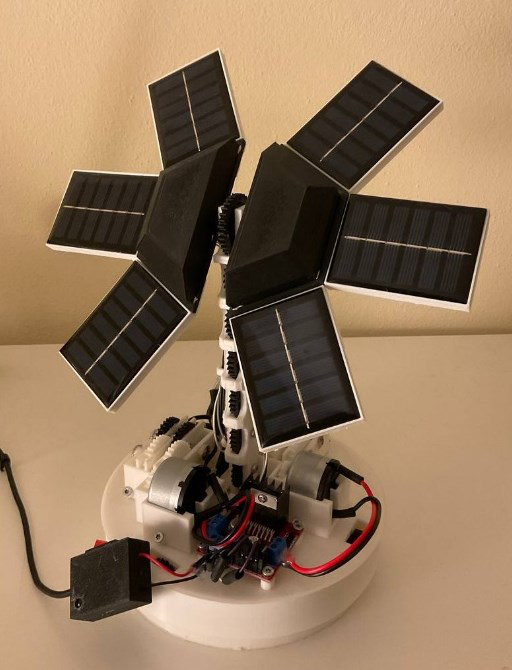
\includegraphics[width=0.8\columnwidth]{final-build}
  \caption{The completed Sunflower robot, connected to the modified power supply.}
  \label{fig:final-build}
\end{figure}

The limitations of the delivered build are the following.

\begin{itemize}
  \item \textbf{No directional awareness.} The single aggregated channel tells the robot whether it is getting better or worse, not which way to go. It therefore has to try a direction and observe the outcome, where the differential two-panel scheme could have pointed straight at the source.
  \item \textbf{Noisy control signal.} With the passive filters removed and only software filtering in place, the signal driving the controller remains noisy.
  \item \textbf{Slipping vertical gear.} Wear on the inner bore of the pistil gear lets the axis slip during up and down rotations. The replacement gear was not reprinted, so the slip remains in the delivered build.
  \item \textbf{Frozen firmware.} Further refinement of the algorithm was cut short when the programmer module of the soldered Arduino failed.
\end{itemize}

\section{Conclusions}
\label{sec:concl}

The project met its objective: a robot, built from stock parts and 3D-printed mechanics, that searches for and tracks a light source on two axes and stops on the maximum.

Two lessons carry beyond this build.

\textbf{Design for disassembly.} A modular approach to the connections, between the printed bodies and between the wires, would have paid for itself several times over. Soldering was expensive, desoldering was worse, and replacing a damaged component meant undoing work that was never designed to be undone. The single most damaging fault in the project, the destroyed filter capacitor, was expensive precisely because the build could not be taken apart.

\textbf{Instrument the analogue path.} An oscilloscope would have exposed both the failing power supply and the capacitive behaviour of the panel immediately. Diagnosing an analogue fault through an Arduino ADC and a serial plotter is guesswork, and it consumed a large share of the effort available for the electronics.

Natural extensions are a charging module with rechargeable batteries, which would make the device self-powered, and weatherproofing with the compensations that outdoor operation requires.

\end{document}
